% This is a Basic Assignment Paper but with like Code and stuff allowed in it, there is also url, hyperlinks from contents included. 

\documentclass[11pt]{article}

% Preamble
\usepackage{multicol}
\usepackage[margin=1in]{geometry}
\usepackage{amsfonts, amsmath, amssymb, amsthm}
\usepackage{fancyhdr, float, graphicx}
\usepackage[utf8]{inputenc} % Required for inputting international characters
\usepackage[T1]{fontenc} % Output font encoding for international characters
\usepackage{fouriernc} % Use the New Century Schoolbook font
\usepackage[nottoc, notlot, notlof]{tocbibind}
\usepackage{listings}
\usepackage{xcolor}
\usepackage{blindtext}
\usepackage{hyperref}
\definecolor{codepurple}{rgb}{0.58,0,0.82}
\hypersetup{
    colorlinks=true,
    linkcolor=black,
    filecolor=black,      
    urlcolor=codepurple,
    pdfpagemode=FullScreen,
    }

\definecolor{codegreen}{rgb}{0,0.6,0}
\definecolor{codegray}{rgb}{0.5,0.5,0.5}
\definecolor{backcolour}{rgb}{0.95,0.95,0.92}

\lstdefinestyle{mystyle}{
    backgroundcolor=\color{backcolour},   
    commentstyle=\color{codegreen},
    keywordstyle=\color{magenta},
    numberstyle=\tiny\color{codegray},
    stringstyle=\color{codepurple},
    basicstyle=\ttfamily\footnotesize,
    breakatwhitespace=false,         
    breaklines=true,                 
    captionpos=b,                    
    keepspaces=true,                 
    numbers=left,                    
    numbersep=5pt,                  
    showspaces=false,                
    showstringspaces=false,
    showtabs=false,                  
    tabsize=2
}

\lstset{style=mystyle}

% Header and Footer
\pagestyle{fancy}
\fancyhead{}
\fancyfoot{}
\fancyhead[L]{\textit{\Large{Mini Project}}}
\fancyhead[R]{\textit{Group A1}}
\fancyfoot[C]{\thepage}
\renewcommand{\footrulewidth}{1pt}
\newtheorem{thm}{Theorem}
\newtheorem{dfn}[thm]{Definition}


% Other Doc Editing
% \parindent 0ex
%\renewcommand{\baselinestretch}{1.5}

\begin{document}

\begin{titlepage}
    \centering

    %---------------------------NAMES-------------------------------

    \begin{figure}[H]
        \centering
        
\includegraphics[width=.75\textwidth]{mitwpu.jpg}
    \end{figure}

    \huge\textsc{
        School of Computer Science and Engineering\\
    }
    \vspace{0.75\baselineskip}
    \Large\textsc{
        Department of Computer Engineering and Technology
    }\\
        \vspace{0.75\baselineskip} % space after Uni Name

    \LARGE{
        Mini Project\\
        Third Year B. Tech, Semester 6
    }

    \vfill % space after Sub Name

    %--------------------------TITLE-------------------------------

    \rule{\textwidth}{1.6pt}\vspace*{-\baselineskip}\vspace*{2pt}
    \rule{\textwidth}{0.6pt}
    \vspace{0.75\baselineskip} % Whitespace above the title



    \huge{\textsc{
        Project Synopsis for\\
        \textbf{ML Powered Facial Attendance Tracking System}
        }} \\



    \vspace{0.5\baselineskip} % Whitespace below the title
    \rule{\textwidth}{0.6pt}\vspace*{-\baselineskip}\vspace*{2.8pt}
    \rule{\textwidth}{1.6pt}

    \vspace{1\baselineskip} % Whitespace after the title block

    %--------------------------SUBTITLE --------------------------	

    \LARGE\textsc{
        Software Development, Machine Learning, AI\\
    } % Subtitle or further description
    \vfill

    %--------------------------AUTHOR-------------------------------

    Prepared By
    \vspace{0.5\baselineskip} % Whitespace before the editors

    \Large{
        PA10. Krishnaraj Thadesar - 1032210888\\
        PA07. Parth Zarekar - 1032210846\\
        PA25. Sourab Karad - 1032211150\\
        PA24. Saubhagya Singh - 1032211144\\
        Cyber Security and Forensics\\
    }


    \vspace{0.5\baselineskip} % Whitespace below the editor list
    2024

\end{titlepage}


\tableofcontents
\thispagestyle{empty}
\clearpage

\setcounter{page}{1}
\begin{multicols}{2}

\section{Abstract}
The "Attendance Assistant" presents a forward-thinking solution for revolutionizing conventional attendance tracking in educational settings. Integrating cloud services such as Amazon S3, Amazon EC2, and Amazon DynamoDB with the official Raspberry Pi High-Quality Camera, the project offers a sophisticated hybrid architecture for efficient and scalable face recognition capabilities.\\

In the cloud infrastructure, Amazon S3 acts as the secure repository for images captured by the Raspberry Pi High-Quality Camera, facilitating organized storage and seamless integration with other AWS services. Amazon EC2 instances play a crucial role in managing continuous processes, serving as the backbone for route management and backend operations. Amazon DynamoDB, a fully managed NoSQL database, anchors the system, efficiently handling dynamic client data and recognition results.\\

At the edge, the Raspberry Pi High-Quality Camera handles real-time image capture, working in tandem with the Raspberry Pi as the edge computing device. This dynamic combination ensures preliminary image processing tasks are executed seamlessly, allowing for real-time interaction with the local environment.\\

The "Attendance Assistant" represents a significant leap towards modernizing attendance tracking processes. By adopting a hybrid architecture that blends the strengths of cloud services with edge computing, the project offers flexibility and scalability, catering to the evolving demands of attendance management in educational institutions.

\subsection*{Keywords}
Facial Recognition and Machine Learning, Artificial Intelligence Integration, Big Data Analysis and Attendance Tracking, Hybrid Architecture with Cloud Services, Cloud Services - AWS, Edge Computing with Raspberry Pi High-Quality Camera, Automated Attendance and Modernization, Educational Technology Integration, Scalability and Efficiency, Real-time Image Capture and Processing, NoSQL Database for Data Management, AWS Services Integration, section{Project Objectives}

\section{Objectives}

\begin{enumerate}
    \item Develop an automated attendance tracking system using computer vision for MITWPU Campus.
    
    \item Utilize cloud infrastructure for efficient storage and processing of attendance data.

    \item Create a user-friendly application for both teachers and students to simplify attendance management.

    \item Implement advanced data science techniques for processing large attendance datasets and performing analytics.

    \item Significantly reduce per-class time spent on attendance tracking through automated processes, enhancing overall efficiency.

    \item Mitigate the risk of malpractices in attendance tracking by implementing secure and tamper-resistant mechanisms.
\end{enumerate}

\section{Hardware and Software Requirements}

\subsection{Hardware Requirements}
\begin{enumerate}
    \item Raspberry Pi 4 Model B with 2GB RAM
    \item Raspberry Pi High-Quality Camera
    \item Raspberry Pi Camera Module 3
    \item Micro SD Card
    \item Power Supply
    \item Internet Connection
    
\end{enumerate}
\end{multicols}

\begin{table}[H]
\centering
    \begin{tabular}{|l|l|l|}
    \hline
    \textbf{Name}                          & \textbf{Purpose}                                                                                                                  & \textbf{Cost} \\ \hline
    Raspberry Pi Hi Quality Camera         & \begin{tabular}[c]{@{}l@{}}Official camera from \\ Raspberry Pi, more expensive \\ for High resolution.\end{tabular}              & 8000          \\ \hline
    Raspberry Pi Camera Module 3           & \begin{tabular}[c]{@{}l@{}}Official camera from \\ Raspberry Pi cheaper and highest \\ resolution for cheapest cost.\end{tabular} & 3000          \\ \hline
    Raspberry PI 4   Model B with 2 GB RAM & To send image from camera to server.                                                                                              & 5000          \\ \hline
    \end{tabular}
    \caption{Hardware Requirements}
    \end{table}

    \begin{multicols}{2}
\subsection{Software Requirements}

\subsubsection{Amazon S3 (Simple Storage Service):}
Amazon S3 serves as the central cloud storage solution for our facial recognition project. Its secure, scalable, and organized storage infrastructure accommodates images captured by the Raspberry Pi High-Quality Camera connected to Raspberry Pi. S3's versatile bucket structure facilitates efficient organization of images and associated metadata, enabling seamless integration with other AWS services.

\subsubsection{Amazon EC2 (Elastic Compute Cloud):}
Amazon EC2 instances play a pivotal role in handling continuous, long-running processes essential for route management and backend operations. Offering a customizable and scalable computing environment, EC2 instances efficiently manage client routes, coordinate responses, and serve as the backbone for the facial recognition application.

\subsubsection{Amazon DynamoDB:}
Amazon DynamoDB, a fully managed NoSQL database, serves as the cornerstone for storing dynamic client data, images, and recognition results. Leveraging DynamoDB's scalability and low-latency access, the system efficiently manages diverse and dynamic data associated with facial recognition.

\subsubsection{Raspberry Pi OS:}
The hardware components, Raspberry Pi High-Quality Camera, and Raspberry Pi form the edge computing segment of the project. The Raspberry Pi High-Quality Camera, equipped with a high-quality camera module, interfaces seamlessly with the Raspberry Pi to capture crisp facial images. The Raspberry Pi, acting as an edge computing device, executes preliminary image processing tasks and ensures real-time interaction with the local environment. We need an raspberry Pi compatible OS to operate these. This also includes Python. 

\end{multicols}

\section{Cost Estimates from AWS}

\begin{figure}[H]
    \centering
    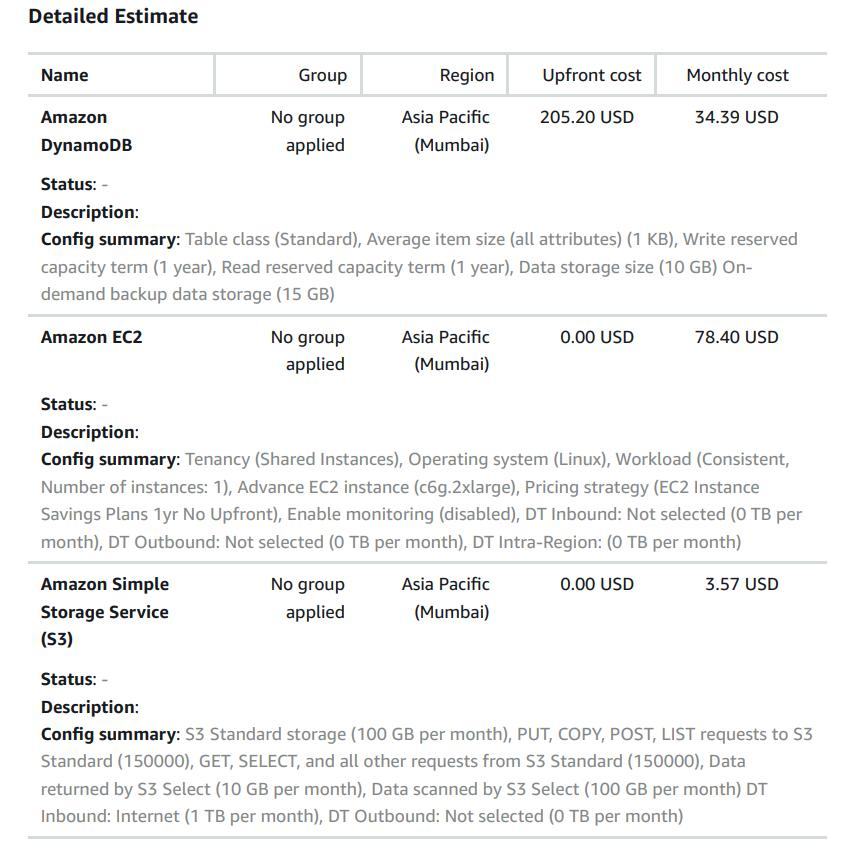
\includegraphics[width=.95\textwidth]{aws estimate.jpg}
    \caption{Estimate from AWS}
\end{figure}

\section{Activity Diagram}
\begin{figure}[H]
    \centering
    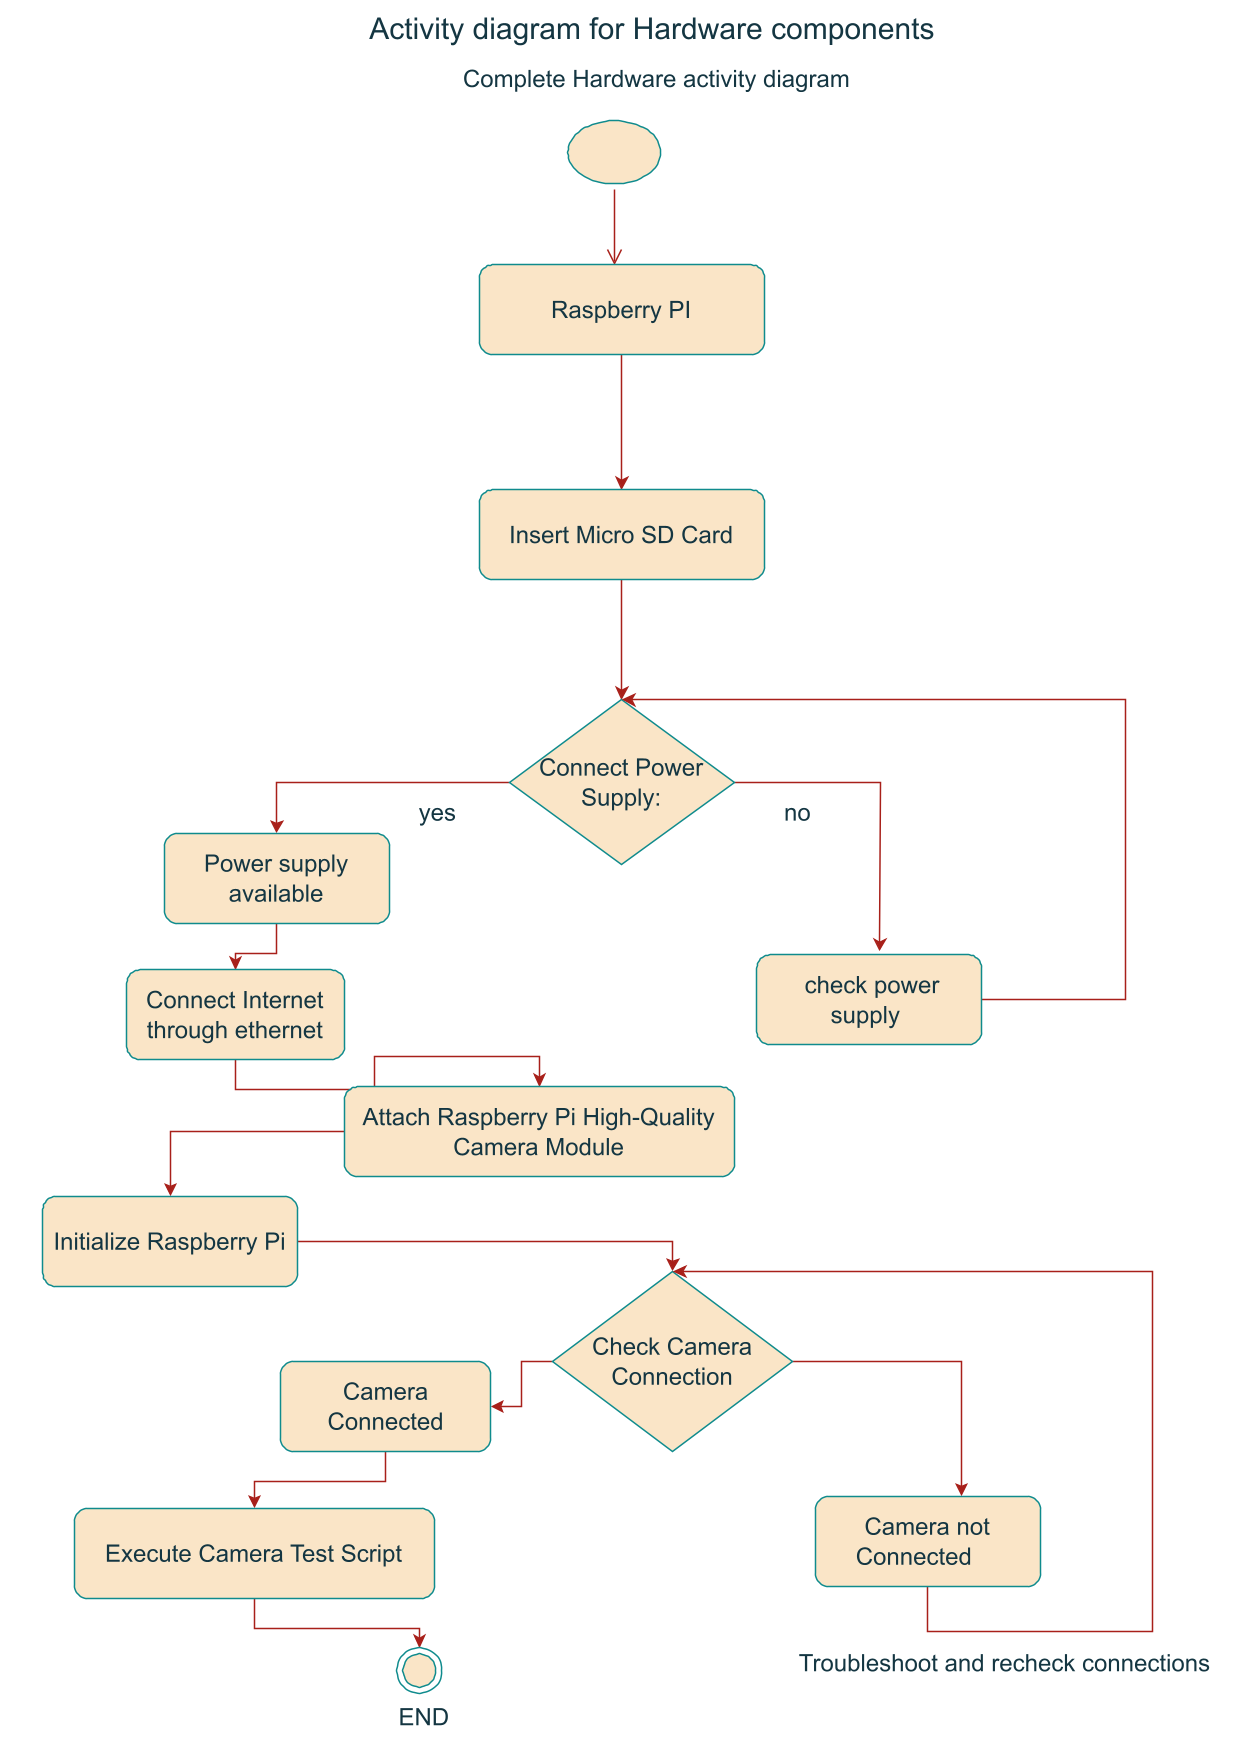
\includegraphics[width=.90\textwidth]{activity_AA.drawio-1.png}
\end{figure}
\begin{figure}[H]
    \centering
    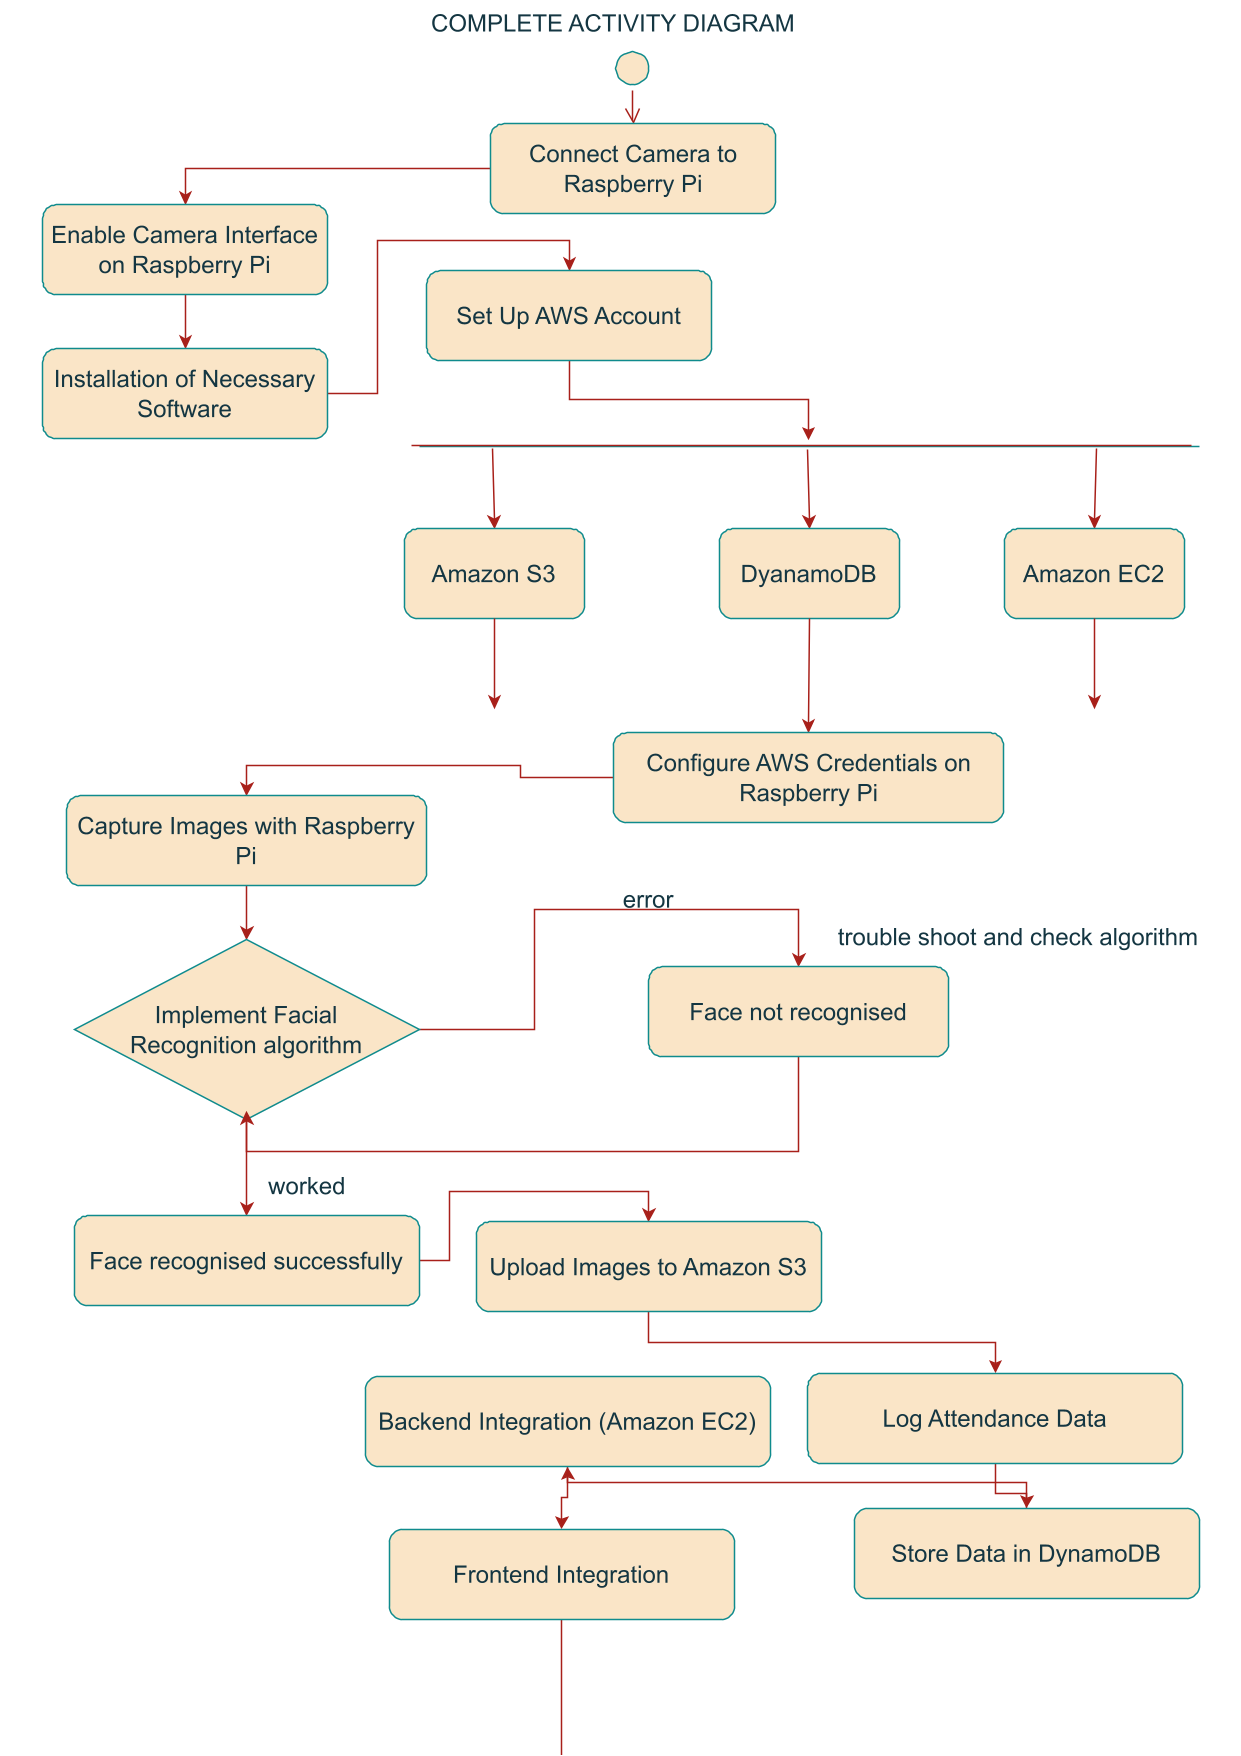
\includegraphics[width=.90\textwidth]{activity_AA.drawio-2.png}
\end{figure}
\begin{figure}[H]
    \centering
    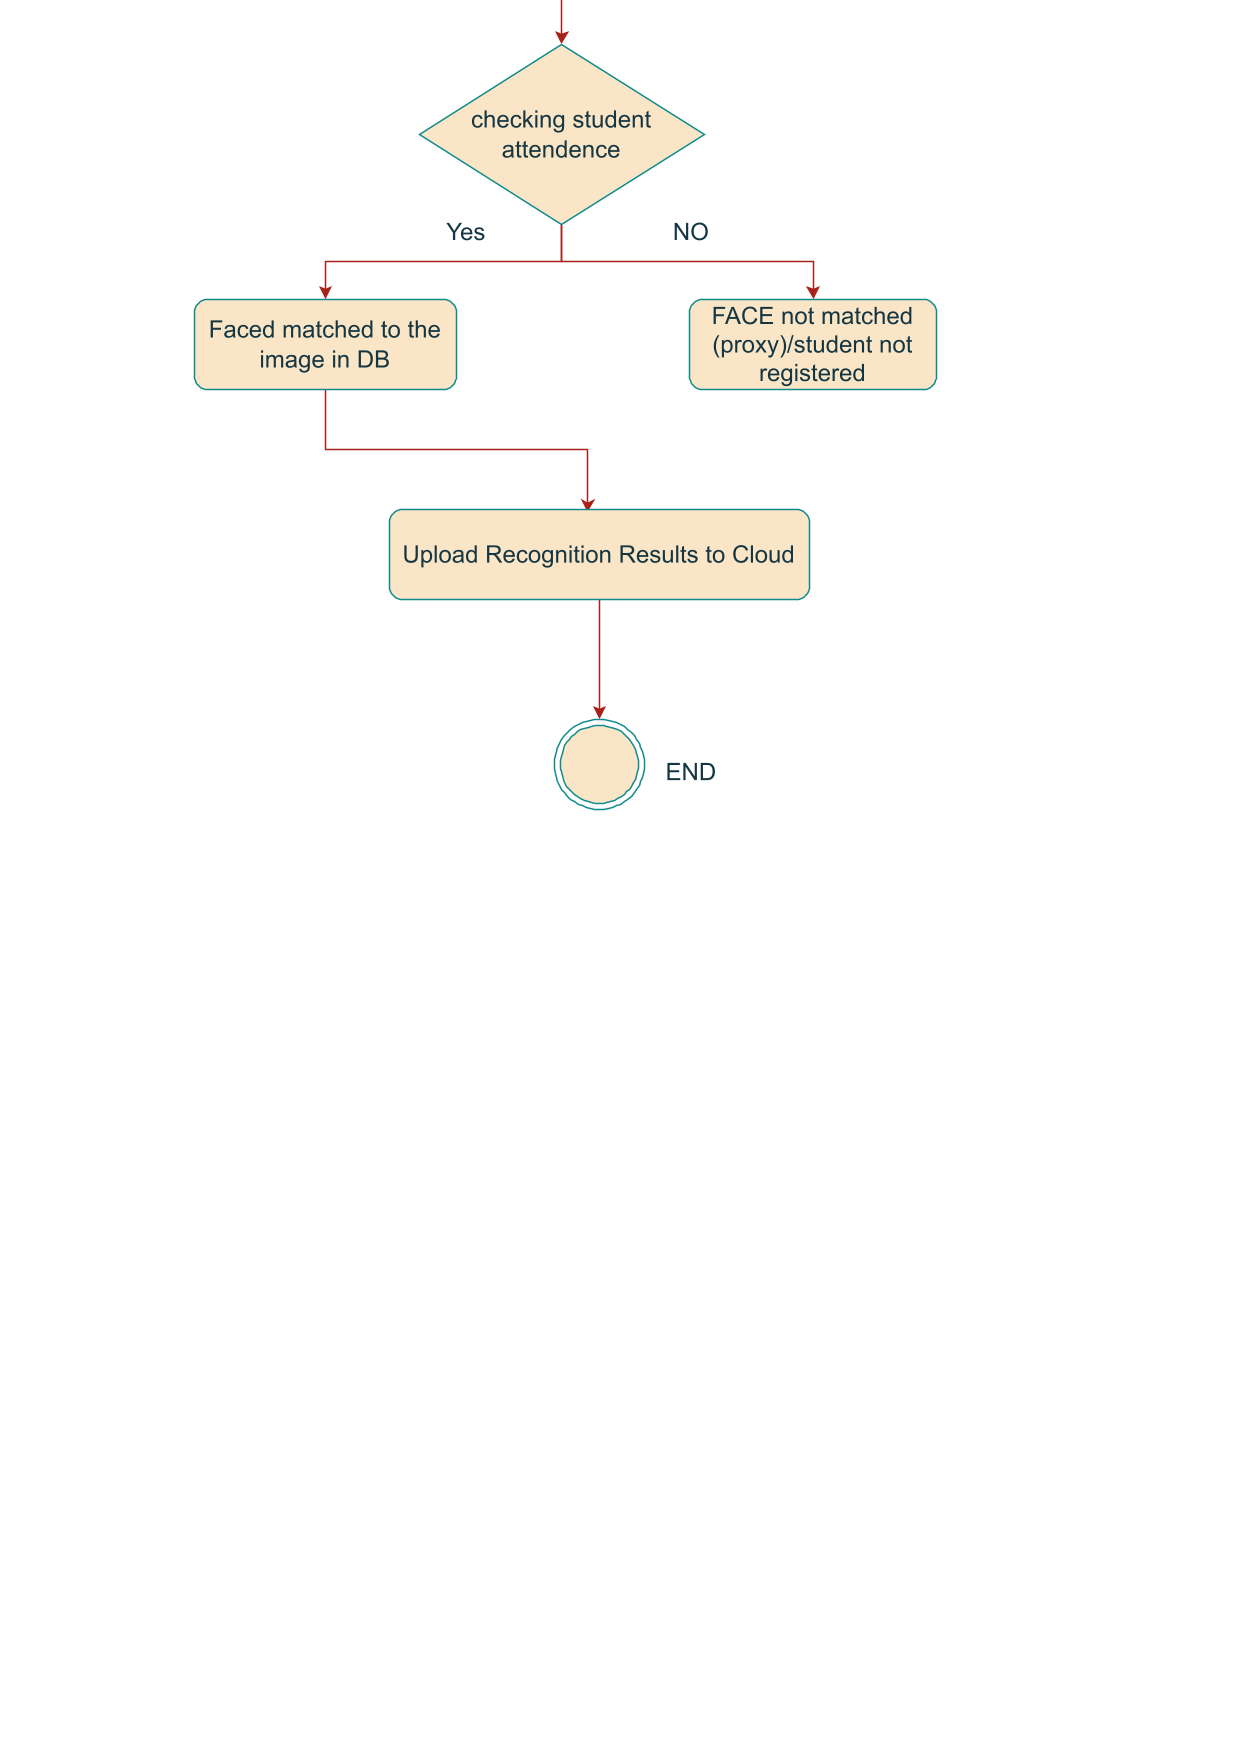
\includegraphics[width=.90\textwidth]{activity_AA.drawio-3.png}
\end{figure}

\section{Block Diagram}
\begin{figure}[H]
    \centering
    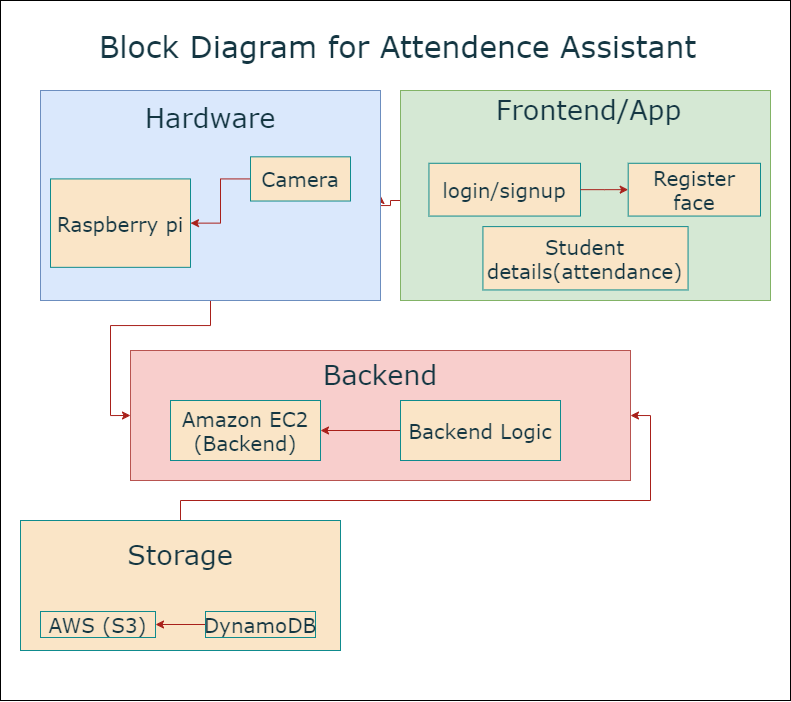
\includegraphics[width=.95\textwidth]{block diagram.png}
\end{figure}

\vfill
\begin{minipage}[t]{0.5\textwidth}
    \raggedright
    \textbf{Mini Project Guide / Mentor}\\
    \vspace*{1cm}
    \textbf{Name}\\
    \vspace*{0.5cm}
    \textbf{Signature}
\end{minipage}%
\hfill
\begin{minipage}[t]{0.5\textwidth}
    \raggedright
    \textbf{Member 1: PA10. Krishnaraj Thadesar }\\
    \vspace*{0.9cm}
    \textbf{Member 2: PA07. Parth Zarekar}\\
    \vspace*{0.9cm}
    \textbf{Member 3: PA25. Sourab Karad }\\
    \vspace*{0.9cm}
    \textbf{Member 4: PA24. Saubhagya Singh }\\
    \vspace*{0.9cm}
\end{minipage}

\pagebreak

\end{document}